\documentclass[10pt]{article}
\usepackage{rsa_icml_like}
\usepackage{amsmath,amssymb,mathtools}
\usepackage{booktabs}
\usepackage{graphicx}
\usepackage{subcaption}
\usepackage{algorithm}
\usepackage{algpseudocode}
\usepackage{tikz}
\usetikzlibrary{arrows.meta,positioning,fit}
\usepackage{pgfplots}
\usepgfplotslibrary{groupplots}
\pgfplotsset{compat=1.18}
\usepackage{multirow}
\usepackage{enumitem}
\usepackage{balance}

\newcommand{\rsa}{\textsc{RSA}}
\newcommand{\code}[1]{\texttt{#1}}
\newcommand{\R}{\mathbb{R}}
\newcommand{\sigmoid}{\sigma}
\newcommand{\logit}{\operatorname{logit}}
\newcommand{\AND}{\mathbin{\wedge}}
\newcommand{\NOT}{\neg}

\title{Random Semantic Algebra: Compiling Latent Search Predicates into Low-Bit Programs}
\author{Hani M. M. Al-Shater\\Independent Research}
\date{September 2026}

\begin{document}

\twocolumn[
\begin{@twocolumnfalse}
\maketitle
\vspace{-1.4em}
\begin{abstract}
Dense retrieval provides an efficient similarity primitive, while structured search provides efficient exact filters; latent constraints such as \emph{minimalist}, \emph{office-appropriate}, or \emph{not sporty} sit awkwardly between them. We introduce \emph{Random Semantic Algebra} (\rsa), which compiles reusable semantic predicates into sparse lookup-table programs over a fixed random 4-bit item code. On a 30k-product mechanism benchmark, a 192-byte/item code preserves the full linear decision boundary almost exactly (0.9334 vs. 0.9331 mean F1), while a sparse 28-coordinate program with four pair interactions reaches 0.9015 mean F1. Calibrated log-probability composition improves two-way conjunction F1 from 0.639 for an earlier soft-box baseline to 0.814 and three-way F1 from 0.476 to 0.747. In a stricter cross-modal pilot, MiniLM title embeddings drive retrieval, CLIP image semantics define eight latent predicates, and \rsa learns those predicates only through the MiniLM-side code; for \emph{minimalist black office shoes not sporty}, retaining 40\% of candidates raises recall from 0.420 to 0.652 and purity from 0.492 to 0.763 at the same downstream budget. These results are preliminary, but they support a systems hypothesis: expensive semantic supervision can be compiled offline into composable, hardware-cheap search operators.
\end{abstract}
\vspace{0.7em}
\end{@twocolumnfalse}
]

\section{Introduction}
Modern search engines expose two mature computational languages. Dense retrieval expresses semantic similarity through inner products or cosine similarity. Structured retrieval expresses exact predicates---brand, size, category, availability---through inverted indexes, bitmaps, or relational filters. A large class of useful constraints is neither: \emph{minimalist}, \emph{office-appropriate}, \emph{technical}, \emph{quiet luxury}, and explicit negations such as \emph{not sporty} are semantic judgments rather than stored facts.

A dense query vector can absorb these words into one score, but logical composition becomes implicit. At the other extreme, a large VLM or LLM can evaluate each predicate directly, but per-candidate model inference inside a retrieval loop is expensive. Recent semantic-operator systems and semantic-filter cascades make this execution problem explicit \citep{patel2025lotus,kim2026semanticfilter,dong2026compilation}.

We study a third design point: \emph{compile once, execute cheaply}. Items are mapped once into a concept-independent low-bit code. Each semantic concept is learned offline as a tiny program over that code. Query understanding then selects and composes already-compiled predicates, leaving dense retrieval and downstream ranking unchanged.

\begin{figure*}[t]
\centering
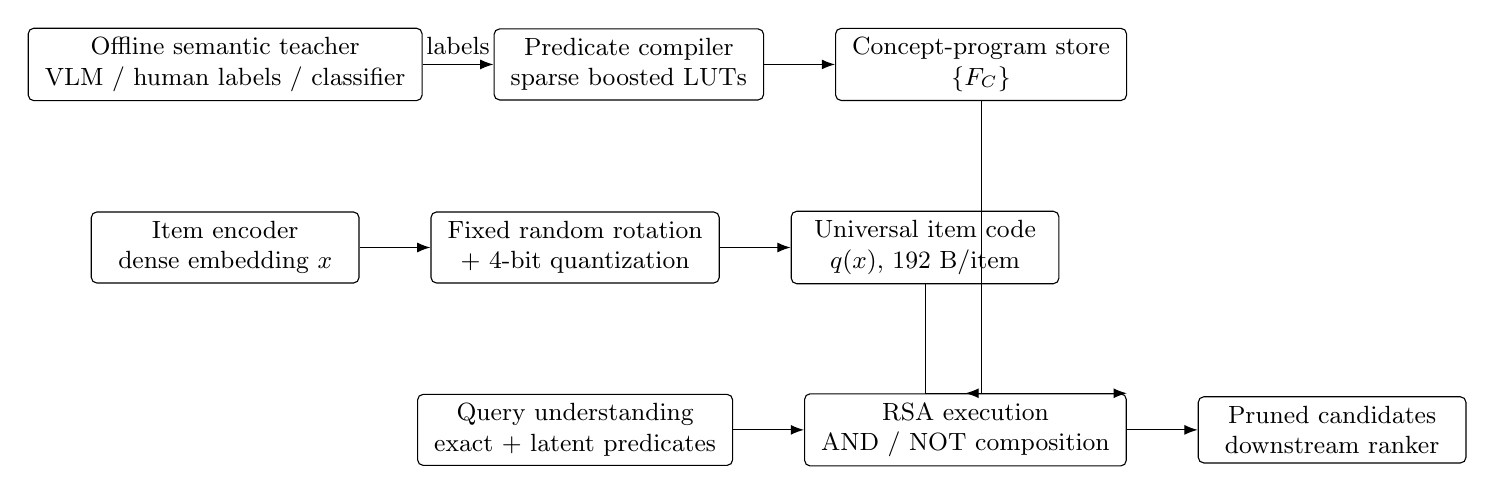
\begin{tikzpicture}[node distance=8mm and 9mm, >=Latex, every node/.style={font=\small}]
\tikzstyle{box}=[draw, rounded corners=2pt, minimum height=8mm, align=center, inner xsep=6pt]
\tikzstyle{big}=[box, minimum width=34mm]
\node[big] (teacher) {Offline semantic teacher\\VLM / human labels / classifier};
\node[big, right=of teacher] (compile) {Predicate compiler\\sparse boosted LUTs};
\node[big, right=of compile] (store) {Concept-program store\\$\{F_C\}$};
\draw[->] (teacher) -- node[above]{labels} (compile);
\draw[->] (compile) -- (store);

\node[big, below=14mm of teacher] (item) {Item encoder\\dense embedding $x$};
\node[big, right=of item] (codebox) {Fixed random rotation\\+ 4-bit quantization};
\node[big, right=of codebox] (code) {Universal item code\\$q(x)$, 192 B/item};
\draw[->] (item) -- (codebox);
\draw[->] (codebox) -- (code);

\node[big, below=14mm of codebox] (query) {Query understanding\\exact + latent predicates};
\node[big, right=of query] (exec) {RSA execution\\AND / NOT composition};
\node[big, right=of exec] (rank) {Pruned candidates\\downstream ranker};
\draw[->] (query) -- (exec);
\draw[->] (store.south) |- (exec.north);
\draw[->] (code.south) |- (exec.north east);
\draw[->] (exec) -- (rank);
\end{tikzpicture}
\caption{\rsa separates expensive semantic supervision from online execution. Exact catalog predicates remain conventional filters; latent predicates are compiled offline into sparse programs over a shared low-bit item code.}
\label{fig:architecture}
\end{figure*}

Our contributions are fourfold. (1) We formulate a concept-independent 4-bit random substrate for reusable semantic predicates. (2) We introduce a residual Newton-boosted compiler that learns sparse one-dimensional lookup functions with optional pair interactions. (3) We show that calibration is the key to composition: conjunction is well approximated by addition of log probabilities, with negation implemented by complement probability. (4) We demonstrate a strict independent-teacher search pilot in which MiniLM retrieves, CLIP images define latent semantics, and \rsa improves candidate quality at fixed budgets.

We do \emph{not} claim that random codes replace ANN retrieval. Our working systems interpretation is narrower: \rsa is a semantic execution layer between broad retrieval and expensive ranking.

\section{Problem Setting}
Let $x\in\R^D$ be a normalized item embedding and $q$ a query embedding. Dense retrieval scores $q^\top x$. Exact predicates, denoted $E(x)$, are stored catalog facts and should remain conventional filters. A \emph{latent predicate} $C$ is a binary semantic judgment supplied by a teacher $T_C(x)\in\{0,1\}$, where the teacher may be a VLM, human annotation process, or specialized model.

The target is a compiler that maps labeled examples into a cheap executable object $F_C$, while keeping the item representation fixed across concepts. We seek: (i) no catalog re-encoding when adding a concept; (ii) low per-item storage; (iii) tens rather than hundreds of arithmetic operations per concept; and (iv) composition of independently learned concepts without conjunction-specific training.

\section{Random Semantic Algebra}
\subsection{Fixed random 4-bit substrate}
Sample a Gaussian matrix and take its orthogonal factor $R\in\R^{D\times D}$. For every item,
\begin{equation}
    z = xR, \qquad q_j = Q_j(z_j)\in\{0,\ldots,15\}.
\end{equation}
Before quantization, orthogonality preserves inner products and Euclidean distances exactly. The prototype learns per-coordinate quantization boundaries on the fit set. For $D=384$, a packed code costs $384\times4/8=192$ bytes/item, versus 1,536 bytes for FP32. This use of randomized low-bit geometry is inspired by work such as random-hyperplane hashing and RaBitQ \citep{charikar2002simhash,gao2024rabitq}; unlike those methods, our target is predicate execution rather than only distance estimation.

\subsection{Sparse predicate programs}
A concept $C$ is represented as
\begin{equation}
F_C(q)=b_C+\sum_{j\in J_C} f_{Cj}(q_j)
+\sum_{(j,k)\in P_C} g_{Cjk}(q_j,q_k),
\label{eq:program}
\end{equation}
where each unary $f_{Cj}$ is a 16-entry table and each optional pair term $g_{Cjk}$ is a $16\times16$ table. This is a discrete, budgeted analogue of a generalized additive model with selected interactions \citep{lou2013ga2m,nori2019interpretml}. Serving cost is dominated by coordinate reads, table lookups, and additions.

\begin{figure}[t]
\centering
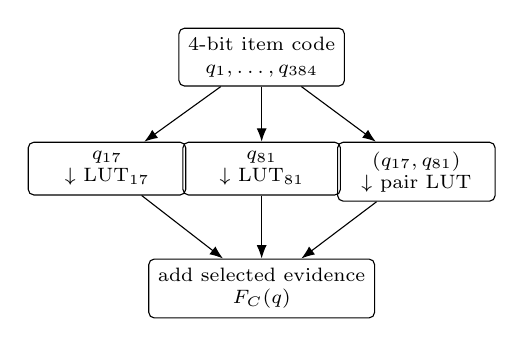
\begin{tikzpicture}[node distance=5mm, >=Latex, every node/.style={font=\scriptsize}]
\tikzstyle{b}=[draw, rounded corners=2pt, align=center, minimum height=6mm, minimum width=20mm]
\node[b] (q) {4-bit item code\\$q_1,\ldots,q_{384}$};
\node[b, below left=7mm and -1mm of q] (u1) {$q_{17}$\\$\downarrow$ LUT$_{17}$};
\node[b, below=7mm of q] (u2) {$q_{81}$\\$\downarrow$ LUT$_{81}$};
\node[b, below right=7mm and -1mm of q] (pair) {$(q_{17},q_{81})$\\$\downarrow$ pair LUT};
\node[b, below=8mm of u2, minimum width=27mm] (sum) {add selected evidence\\$F_C(q)$};
\draw[->] (q) -- (u1); \draw[->] (q) -- (u2); \draw[->] (q) -- (pair);
\draw[->] (u1) -- (sum); \draw[->] (u2) -- (sum); \draw[->] (pair) -- (sum);
\end{tikzpicture}
\caption{A compiled predicate touches only selected coordinates. The search pilot uses 24 unary tables and two pair tables (26 LUT operations/concept).}
\label{fig:predicate}
\end{figure}

\subsection{Residual Newton boosting}
Given current logits $s_i=F_C(q_i)$, let $p_i=\sigmoid(s_i)$, gradient residual $r_i=y_i-p_i$, and curvature $h_i=p_i(1-p_i)$. For candidate coordinate $j$ and bin $v$, define
\begin{equation}
G_{jv}=\sum_{i:q_{ij}=v} r_i,\qquad
H_{jv}=\sum_{i:q_{ij}=v} h_i.
\end{equation}
The Newton table is $\Delta f_j(v)=G_{jv}/(H_{jv}+\lambda)$, with approximate gain
\begin{equation}
\mathcal{G}_j=\frac12\sum_v \frac{G_{jv}^2}{H_{jv}+\lambda}.
\end{equation}
At each stage we add the highest-gain coordinate not yet selected and update residuals. A short cyclic backfitting pass then refits the selected tables. Pair tables are learned analogously over joint $16\times16$ bins.

\begin{algorithm}[t]
\caption{Compile a latent predicate $C$}
\label{alg:compile}
\begin{algorithmic}[1]
\Require Quantized fit codes $Q$, labels $y_C$, unary budget $K$, pair budget $M$
\State $b\gets \logit((\sum_i y_i+0.5)/(n+1))$; $s_i\gets b$
\State Build a candidate pool using marginal discriminative strength
\For{$t=1,\ldots,K$}
  \State $p_i\gets\sigmoid(s_i)$; $r_i\gets y_i-p_i$; $h_i\gets p_i(1-p_i)$
  \For{each candidate coordinate $j$}
    \State compute $\Delta f_j(v)=G_{jv}/(H_{jv}+\lambda)$ and gain $\mathcal{G}_j$
  \EndFor
  \State select $j^*=\arg\max_j\mathcal{G}_j$; add $\eta\Delta f_{j^*}$ to $F_C$ and $s$
\EndFor
\State cyclically refit selected unary tables with Newton updates
\For{$m=1,\ldots,M$}
  \State select the highest-gain pair among selected coordinates
  \State add a $16\times16$ pair table $g_{jk}$
\EndFor
\State \Return sparse program $F_C=(b,J_C,\{f_{Cj}\},P_C,\{g_{Cjk}\})$
\end{algorithmic}
\end{algorithm}

\subsection{Calibration and semantic algebra}
Independently trained concept logits are not on a common evidence scale. On a held-out calibration split, fit a scalar map
\begin{equation}
L_C(x)=a_CF_C(q(x))+c_C, \qquad p_C(x)=\sigmoid(L_C(x)).
\end{equation}
For positive predicates $\mathcal{Q}^+$ and negated predicates $\mathcal{Q}^-$, we score
\begin{equation}
S_{\mathcal{Q}}(x)=\sum_{C\in\mathcal{Q}^+}\log p_C(x)+
\sum_{C\in\mathcal{Q}^-}\log(1-p_C(x)).
\label{eq:composition}
\end{equation}
This product-of-evidence operator is commutative and associative over the selected predicates, so a query can be assembled from independently compiled concepts. We evaluate AND and NOT; other operators are future work.

\begin{algorithm}[t]
\caption{Execute a semantic query plan}
\label{alg:execute}
\begin{algorithmic}[1]
\Require ANN candidate set $A$, exact filters $E$, positive concepts $\mathcal{Q}^+$, negative concepts $\mathcal{Q}^-$, budget $B$
\State $A'\gets\{x\in A:E(x)=\mathrm{true}\}$
\For{each $x\in A'$}
  \State evaluate only the compiled programs requested by the query
  \State compute $S_{\mathcal{Q}}(x)$ using Eq.~\eqref{eq:composition}
\EndFor
\State retain the $B$ highest-scoring candidates
\State \Return survivors to the downstream ranker
\end{algorithmic}
\end{algorithm}

\section{Experimental Setup}
\paragraph{Dataset.} We use Fashion Product Images Small \citep{fashiondataset}. The exploratory mechanism benchmark samples 30k products; the independent-teacher pilot samples 8k products to keep image encoding practical.

\paragraph{Mechanism benchmark.} Product titles are encoded by MiniLM \citep{reimers2019sbert,wang2020minilm} into 384-dimensional normalized vectors. Fourteen structured fields serve as concept labels. Product titles often contain those labels, so this benchmark is intentionally a representation/compiler mechanism test, not a leakage-free latent-semantic benchmark. Results use the original 65/35 train/test split; binary thresholds are fit on train.

\paragraph{Independent-teacher pilot.} MiniLM title embeddings provide retrieval and the \rsa substrate. CLIP ViT-B/32 image semantics \citep{radford2021clip} independently define eight concepts: minimalist, office-appropriate, technical/sporty, retro, elegant, relaxed, chunky, and quiet luxury. The 8k products are split into 4,160 fit, 1,040 calibration, and 2,800 held-out test items. For each concept, CLIP scores an image against positive and negative prompt sets; a fit-set threshold produces 40\% prevalence and is frozen for calibration/test. \rsa sees only the MiniLM-side 4-bit code.

\paragraph{Search protocol.} MiniLM retrieves the top 500 test items. Exact constraints such as \code{Black} and \code{Shoes} are applied as normal filters. The baseline retains the top $B$ remaining items by dense score. \rsa retains the same $B$ by Eq.~\eqref{eq:composition}, then preserves dense order among survivors. Relevance is the conjunction of exact filters and independent CLIP-derived latent labels.

\section{Results}
\subsection{Sparse programs preserve most classifier quality}
Table~\ref{tab:mechanism} and Figure~\ref{fig:mechanism} summarize the mechanism benchmark. Compiling all 384 coordinates into 4-bit lookup tables matches the FP32 linear teacher within measurement noise, showing that the 4-bit substrate itself is not the principal bottleneck. Sparsifying to 28 unary terms plus four interactions retains 0.9015 mean F1, or 96.6\% of the teacher's F1. The largest gain comes from residual optimization, not interactions: boosted unary LUTs reach 0.8993, whereas independently estimated LLR factors reach 0.8152.

\begin{table}[t]
\centering
\caption{Mechanism benchmark (14 concepts).}
\label{tab:mechanism}
\small
\begin{tabular}{lcc}
\toprule
Method & Mean F1 & Mean AP\\
\midrule
FP32 linear & 0.9331 & 0.9596\\
Compiled linear, 384 LUTs & \textbf{0.9334} & \textbf{0.9596}\\
Boosted LUT + 4 pairs & 0.9015 & 0.9388\\
Boosted unary LUT & 0.8993 & 0.9372\\
Compiled linear, 28 coords & 0.8619 & 0.9102\\
LLR + EB + mRMR & 0.8346 & 0.8902\\
LLR factor & 0.8152 & 0.8724\\
\bottomrule
\end{tabular}
\end{table}

\begin{figure}[t]
\centering
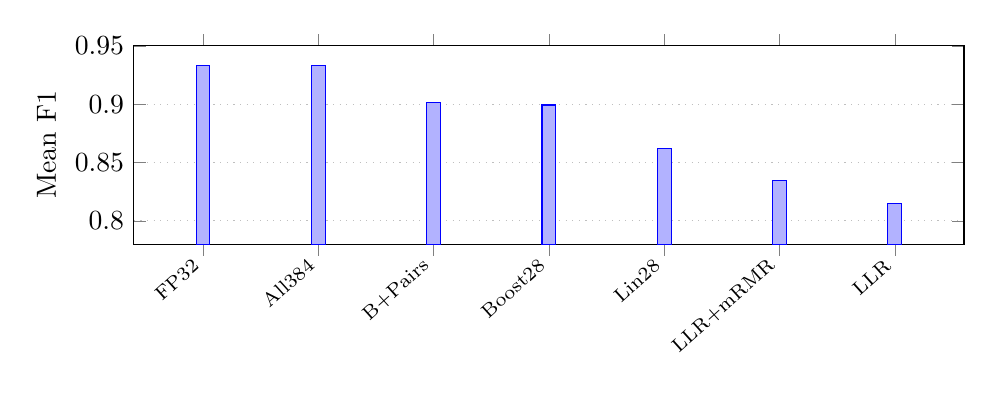
\begin{tikzpicture}
\begin{axis}[
  width=\columnwidth,height=4.1cm,
  ybar, ymin=0.78,ymax=0.95,
  ylabel={Mean F1},
  symbolic x coords={FP32,All384,B+Pairs,Boost28,Lin28,LLR+mRMR,LLR},
  xtick=data, x tick label style={rotate=42,anchor=east,font=\scriptsize},
  ymajorgrids=true, grid style={dotted},
  bar width=5pt,
]
\addplot coordinates {(FP32,0.9331) (All384,0.9334) (B+Pairs,0.9015) (Boost28,0.8993) (Lin28,0.8619) (LLR+mRMR,0.8346) (LLR,0.8152)};
\end{axis}
\end{tikzpicture}
\caption{Residual-optimized LUTs close most of the gap to the full-precision linear classifier.}
\label{fig:mechanism}
\end{figure}

\paragraph{Ablations.} At a fixed 192-byte item budget, 384 four-bit coordinates outperform 768 two-bit coordinates (0.8993 vs. 0.8894 mean F1) and 1,536 one-bit random directions (0.8630). Power whitening consistently hurts: $\gamma=0.25,0.5,0.75,1.0$ produce 0.8944, 0.8654, 0.7993, and 0.6881 F1 respectively. Uniform and quantile 4-bit bins are effectively tied. These results suggest that pretrained-embedding anisotropy is useful signal for sparse predicate compilation rather than nuisance variation.

\subsection{Calibration changes the composition regime}
Raw addition of independently trained logits performs poorly, especially for three-way conjunctions. After scalar calibration, several soft AND rules converge to similar quality; the simple log-probability product is preferred because it is algebraically clean and requires no conjunction-specific model.

\begin{table}[t]
\centering
\caption{Composition of independently learned predicates.}
\label{tab:composition}
\small
\begin{tabular}{lcc}
\toprule
Rule & 2-way F1 & 3-way F1\\
\midrule
Raw logit add & 0.7148 & 0.5633\\
Min calibrated logit & 0.8140 & 0.7428\\
Log-probability product & \textbf{0.8142} & 0.7459\\
Soft-min ($\tau=1$) & 0.8141 & 0.7451\\
Correlation weighted & 0.8142 & \textbf{0.7470}\\
\bottomrule
\end{tabular}
\end{table}

\begin{figure}[t]
\centering
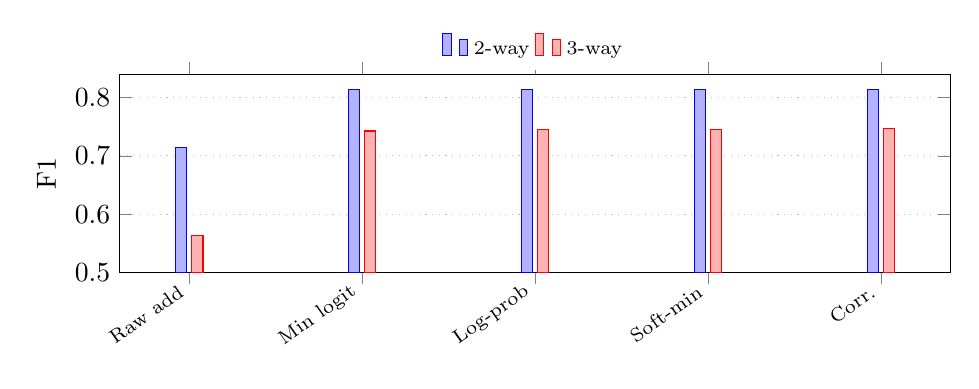
\begin{tikzpicture}
\begin{axis}[
  width=\columnwidth,height=4.1cm,
  ybar, ymin=0.5,ymax=0.84,
  ylabel={F1},
  symbolic x coords={Raw,Min,LogP,Soft,Corr}, xtick=data,
  xticklabels={Raw add,Min logit,Log-prob,Soft-min,Corr.},
  x tick label style={rotate=35,anchor=east,font=\scriptsize},
  legend style={font=\scriptsize,draw=none,at={(0.5,1.02)},anchor=south,legend columns=2},
  ymajorgrids=true, grid style={dotted}, bar width=4pt,
]
\addplot coordinates {(Raw,0.7148) (Min,0.8140) (LogP,0.8142) (Soft,0.8141) (Corr,0.8142)};
\addplot coordinates {(Raw,0.5633) (Min,0.7428) (LogP,0.7459) (Soft,0.7451) (Corr,0.7470)};
\legend{2-way,3-way}
\end{axis}
\end{tikzpicture}
\caption{Calibration, rather than a complex combination rule, drives the improvement in semantic conjunction.}
\label{fig:composition}
\end{figure}

The earlier geometric formulation obtained 0.639 F1 for two-way soft AND and 0.476 for three-way literal boxes. The calibrated program algebra reaches about 0.814 and 0.746--0.747, indicating that independently learned predicates remain useful together when statistical evidence is not treated as hard geometry.

\subsection{Cross-modal latent predicate compilation}
The independent-teacher experiment is intentionally harder: the teacher sees images while \rsa sees only title-derived MiniLM codes. Table~\ref{tab:latent} shows a mean F1 of 0.689 and AP of 0.725 using 26 LUT operations per concept. Transfer varies substantially by concept; quiet luxury transfers best, while retro and chunky expose missing or weak title-side information.

\begin{table}[t]
\centering
\caption{Held-out transfer from CLIP image semantics to title-side RSA programs.}
\label{tab:latent}
\small
\begin{tabular}{lcc}
\toprule
Concept & F1 & AP\\
\midrule
Quiet luxury & 0.776 & 0.866\\
Elegant & 0.730 & 0.768\\
Minimalist & 0.702 & 0.772\\
Technical/sporty & 0.690 & 0.688\\
Office appropriate & 0.677 & 0.731\\
Relaxed & 0.671 & 0.658\\
Retro & 0.637 & 0.672\\
Chunky & 0.627 & 0.646\\
\midrule
Mean & \textbf{0.689} & \textbf{0.725}\\
\bottomrule
\end{tabular}
\end{table}

\begin{figure}[t]
\centering
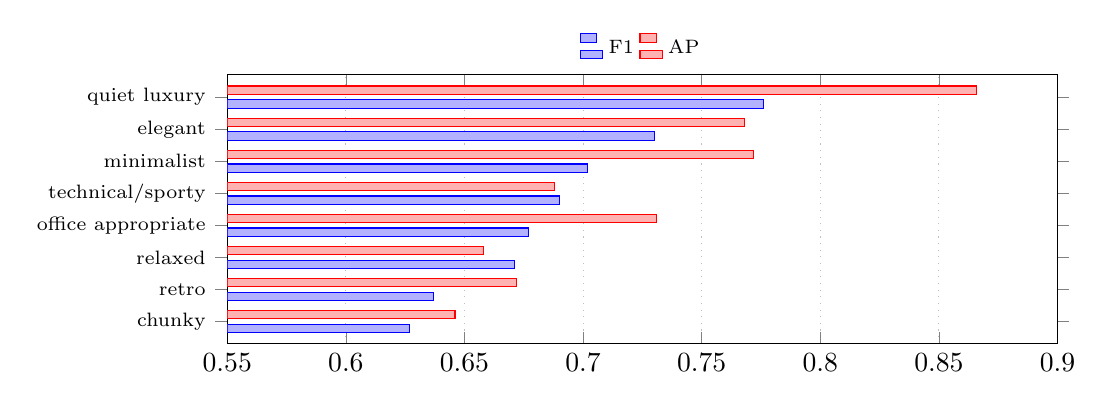
\begin{tikzpicture}
\begin{axis}[
  width=\columnwidth,height=5.0cm,
  xbar, xmin=0.55,xmax=0.9,
  symbolic y coords={Chunky,Retro,Relaxed,Office,Technical,Minimalist,Elegant,Quiet},
  ytick=data,
  yticklabels={chunky,retro,relaxed,office appropriate,technical/sporty,minimalist,elegant,quiet luxury},
  y tick label style={font=\scriptsize},
  legend style={font=\scriptsize,draw=none,at={(0.5,1.02)},anchor=south,legend columns=2},
  xmajorgrids=true, grid style={dotted}, bar width=3pt,
]
\addplot coordinates {(0.627,Chunky) (0.637,Retro) (0.671,Relaxed) (0.677,Office) (0.690,Technical) (0.702,Minimalist) (0.730,Elegant) (0.776,Quiet)};
\addplot coordinates {(0.646,Chunky) (0.672,Retro) (0.658,Relaxed) (0.731,Office) (0.688,Technical) (0.772,Minimalist) (0.768,Elegant) (0.866,Quiet)};
\legend{F1,AP}
\end{axis}
\end{tikzpicture}
\caption{Cross-modal predicate transfer quality. CLIP image labels are predicted using only the 4-bit code derived from MiniLM titles.}
\label{fig:latent}
\end{figure}

\subsection{Fixed-budget candidate pruning}
For the query \emph{minimalist black office shoes not sporty}, MiniLM retrieves 500 items and exact Black/Shoes filters leave 147 candidates, of which 69 satisfy the CLIP-defined latent conjunction. Figure~\ref{fig:retention} shows the candidate-budget frontier. At 40\% retention (59 candidates), dense truncation keeps 29 relevant items (0.420 recall, 0.492 purity), while \rsa keeps 45 (0.652 recall, 0.763 purity): 55\% more relevant items for the same downstream budget. At 10\% retention, \rsa reaches 0.933 purity and keeps 14 of 15 candidates relevant.

\begin{table}[t]
\centering
\caption{Independent-teacher search pilot at matched candidate budgets.}
\label{tab:retention}
\small
\begin{tabular}{rcccc}
\toprule
Keep & Dense R & RSA R & Dense P & RSA P\\
\midrule
40\% & 0.420 & \textbf{0.652} & 0.492 & \textbf{0.763}\\
20\% & 0.246 & \textbf{0.333} & 0.586 & \textbf{0.793}\\
10\% & 0.159 & \textbf{0.203} & 0.733 & \textbf{0.933}\\
5\%  & 0.087 & \textbf{0.101} & 0.857 & \textbf{1.000}\\
\bottomrule
\end{tabular}
\end{table}

\begin{figure*}[t]
\centering
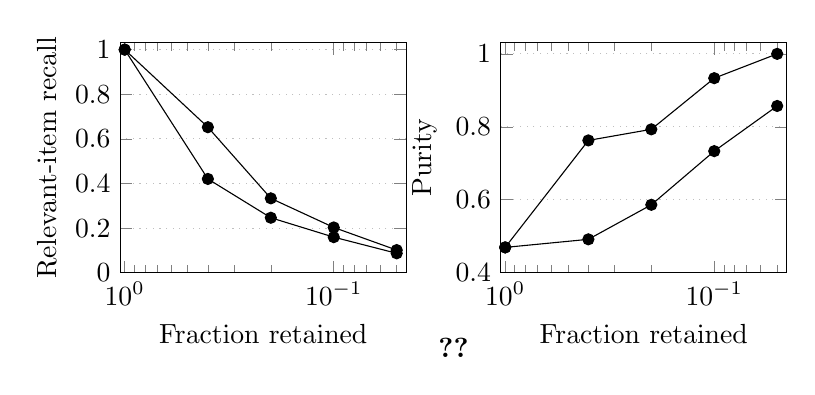
\begin{tikzpicture}
\begin{groupplot}[
  group style={group size=2 by 1,horizontal sep=1.2cm},
  width=0.43\textwidth,height=4.5cm,
  xmode=log, x dir=reverse, xmin=0.045,xmax=1.05,
  xlabel={Fraction retained},
  ymajorgrids=true, grid style={dotted},
  legend style={font=\scriptsize,draw=none},
]
\nextgroupplot[ymin=0,ymax=1.03,ylabel={Relevant-item recall},legend to name=sharedlegend]
\addplot[mark=*] coordinates {(1,1) (.4,.420290) (.2,.246377) (.1,.159420) (.05,.086957)};
\addplot[mark=*] coordinates {(1,1) (.4,.652174) (.2,.333333) (.1,.202899) (.05,.101449)};
\legend{Dense-only,RSA}
\nextgroupplot[ymin=0.4,ymax=1.03,ylabel={Purity}]
\addplot[mark=*] coordinates {(1,.469388) (.4,.491525) (.2,.586207) (.1,.733333) (.05,.857143)};
\addplot[mark=*] coordinates {(1,.469388) (.4,.762712) (.2,.793103) (.1,.933333) (.05,1.0)};
\end{groupplot}
\node at ($(group c1r1.south east)!0.5!(group c2r1.south west)+(0,-0.95cm)$) {\ref{sharedlegend}};
\end{tikzpicture}
\caption{Independent-teacher pilot. \textbf{Left:} recall of CLIP-defined relevant items versus retained candidate fraction. \textbf{Right:} purity of retained candidates. \rsa dominates dense-only truncation at every nontrivial budget for this query.}
\label{fig:retention}
\end{figure*}

\section{Related Work}
\paragraph{Quantized retrieval.} Product Quantization compresses vectors for ANN search \citep{jegou2011pq}; random-hyperplane hashing connects sign agreement to angle \citep{charikar2002simhash}. RaBitQ provides randomized low-bit distance estimation with error bounds \citep{gao2024rabitq}. MUVERA compiles multi-vector similarity into fixed-dimensional encodings for conventional MIPS infrastructure \citep{dhulipala2024muvera}. \rsa shares the compilation philosophy but targets many reusable semantic predicates over a shared item code.

\paragraph{Filtered vector search.} Filtered ANN combines vector similarity with structured predicates and introduces nontrivial recall/latency trade-offs depending on selectivity and correlation \citep{chronis2025filtered}. \rsa is complementary: exact structured predicates should remain native filters; \rsa targets semantic judgments that are not explicit fields.

\paragraph{Semantic operators and proxy execution.} LOTUS formalizes natural-language semantic operators and their optimization \citep{patel2025lotus}. Recent semantic-filter work studies learned proxies and adaptive cascades to reduce expensive oracle calls \citep{kim2026semanticfilter}. Compilation-based semantic execution similarly moves semantic interpretation out of per-item runtime \citep{dong2026compilation}. \rsa occupies a distinct low-level design point: a fixed low-bit item substrate, sparse learned LUT programs, and explicit algebraic composition for retrieval-time execution.

\section{Limitations and Next Experiments}
The present evidence is exploratory. The mechanism benchmark contains lexical leakage and was used for broad method exploration. The independent-teacher retrieval result is one compound query on one fashion dataset, with CLIP prompts rather than human relevance judgments. The prototype stores 4-bit values as NumPy bytes and does not yet implement nibble packing, int8 LUTs, SIMD kernels, cache-aware layouts, or integration with an ANN index. Main results use one random rotation/seed.

The decisive evaluation is therefore a 50--200 query benchmark spanning categories, positive predicates, negations, and selectivities, with independent VLM or human labels and bootstrap confidence intervals. Baselines should include dense-only truncation, sparse and full linear probes, small MLP proxies, additive models on the original dense vector, and semantic-filter cascade methods. The main systems curve should be relevant-item recall (or NDCG) versus retained candidates and measured latency. A packed CPU implementation is needed to establish whether the theoretical low arithmetic count converts into end-to-end savings.

\section{Conclusion}
\rsa explores a semantic-search primitive between similarity and exact filtering. A fixed 4-bit item code can host sparse compiled predicates; residual boosting captures substantially more signal than hard boxes or independent likelihood factors; and calibration enables useful AND/NOT composition without training conjunction-specific representations. In a cross-modal pilot, title-side \rsa programs recover enough CLIP image semantics to improve recall and purity at fixed candidate budgets. The result is not yet a production search claim, but it motivates a concrete research program: move expensive semantic supervision offline and execute its reusable decisions as tiny search-time programs.

\section*{Impact Statement}
If successful at scale, compiled semantic predicates could reduce online model inference and energy use in retrieval systems while enabling richer natural-language constraints. The same mechanism could also encode biased or poorly specified teacher judgments at scale; deployed systems should therefore audit predicate labels, calibration, subgroup behavior, and failure modes, and should preserve conventional safety and policy filters outside the learned semantic layer.

\begin{thebibliography}{99}

\bibitem[J{\'e}gou et~al.(2011)J{\'e}gou, Douze, and Schmid]{jegou2011pq}
H. J{\'e}gou, M. Douze, and C. Schmid. Product Quantization for Nearest Neighbor Search. \emph{IEEE TPAMI}, 33(1):117--128, 2011.

\bibitem[Charikar(2002)]{charikar2002simhash}
M. S. Charikar. Similarity Estimation Techniques from Rounding Algorithms. In \emph{STOC}, pp. 380--388, 2002.

\bibitem[Gao and Long(2024)]{gao2024rabitq}
J. Gao and C. Long. RaBitQ: Quantizing High-Dimensional Vectors with a Theoretical Error Bound for Approximate Nearest Neighbor Search. \emph{arXiv:2405.12497}, 2024.

\bibitem[Dhulipala et~al.(2024)Dhulipala, Hadian, Jayaram, Lee, and Mirrokni]{dhulipala2024muvera}
L. Dhulipala, M. Hadian, R. Jayaram, J. Lee, and V. Mirrokni. MUVERA: Multi-Vector Retrieval via Fixed Dimensional Encodings. In \emph{NeurIPS}, 2024.

\bibitem[Chronis et~al.(2025)Chronis, Caminal, Papakonstantinou, {\"O}zcan, and Ailamaki]{chronis2025filtered}
Y. Chronis, H. Caminal, Y. Papakonstantinou, F. {\"O}zcan, and A. Ailamaki. Filtered Vector Search: State-of-the-Art and Research Opportunities. \emph{PVLDB}, 18(12):5488--5492, 2025.

\bibitem[Patel et~al.(2025)Patel, Jha, Pan, Gupta, Asawa, Guestrin, and Zaharia]{patel2025lotus}
L. Patel, S. Jha, M. Pan, H. Gupta, P. Asawa, C. Guestrin, and M. Zaharia. Semantic Operators and Their Optimization: Enabling LLM-Based Data Processing with Accuracy Guarantees in LOTUS. \emph{PVLDB}, 18(11):4171--4184, 2025.

\bibitem[Kim et~al.(2026)Kim, Catheland, and Ailamaki]{kim2026semanticfilter}
K. Kim, M. Catheland, and A. Ailamaki. Fast LLM-Based Semantic Filtering: From a Unified Framework to an Adaptive Two-Phase Method. \emph{arXiv:2606.08090}, 2026.

\bibitem[Dong and Wang(2026)]{dong2026compilation}
W. Dong and Y. Wang. From Interpretation to Compilation: Compilation-Based Execution of Semantic Operators [Vision]. \emph{arXiv:2607.13407}, 2026.

\bibitem[Lou et~al.(2013)Lou, Caruana, Gehrke, and Hooker]{lou2013ga2m}
Y. Lou, R. Caruana, J. Gehrke, and G. Hooker. Accurate Intelligible Models with Pairwise Interactions. In \emph{KDD}, pp. 623--631, 2013.

\bibitem[Nori et~al.(2019)Nori, Jenkins, Koch, and Caruana]{nori2019interpretml}
H. Nori, S. Jenkins, P. Koch, and R. Caruana. InterpretML: A Unified Framework for Machine Learning Interpretability. \emph{arXiv:1909.09223}, 2019.

\bibitem[Reimers and Gurevych(2019)]{reimers2019sbert}
N. Reimers and I. Gurevych. Sentence-BERT: Sentence Embeddings using Siamese BERT-Networks. In \emph{EMNLP-IJCNLP}, pp. 3982--3992, 2019.

\bibitem[Wang et~al.(2020)Wang, Wei, Dong, Bao, Yang, and Zhou]{wang2020minilm}
W. Wang, F. Wei, L. Dong, H. Bao, N. Yang, and M. Zhou. MiniLM: Deep Self-Attention Distillation for Task-Agnostic Compression of Pre-Trained Transformers. In \emph{NeurIPS}, 2020.

\bibitem[Radford et~al.(2021)]{radford2021clip}
A. Radford et~al. Learning Transferable Visual Models From Natural Language Supervision. In \emph{ICML}, pp. 8748--8763, 2021.

\bibitem[Ashraq(2026)]{fashiondataset}
Ashraq. Fashion Product Images Small. Hugging Face Datasets, accessed 2026.

\end{thebibliography}

\appendix
\section{Additional Experimental Detail}
\subsection{Original geometry sanity check}
The original mechanism run measured correlation 0.9102 between source cosine similarity and 1-bit Hamming agreement, and 0.9761 between source cosine and a 4-bit negative-$\ell_1$ surrogate over random held-out pairs. These values motivate the low-bit substrate but are not ANN recall guarantees.

\subsection{Storage accounting}
For $D=384$, source FP32 embeddings require 1,536 bytes/item. A packed 4-bit substrate requires 192 bytes/item and a packed 1-bit substrate 48 bytes/item. Current NumPy prototypes store codes in \code{uint8}; all storage claims in the paper refer to the packed systems representation. A unary semantic program with 24 active coordinates and 16 int8 values per coordinate requires 384 table bytes plus coordinate identifiers and an intercept; the search pilot adds two $16\times16$ pair tables.

\subsection{Mechanism ablations}
\begin{table}[h]
\centering
\small
\caption{Selected ablations on the 30k mechanism benchmark.}
\begin{tabular}{lc}
\toprule
Configuration & Mean F1\\
\midrule
384$\times$4-bit orthogonal, boosted unary & 0.8993\\
768$\times$2-bit independent dictionary & 0.8894\\
1536$\times$1-bit independent dictionary & 0.8630\\
Power whitening $\gamma=0.25$ & 0.8944\\
Power whitening $\gamma=0.50$ & 0.8654\\
Power whitening $\gamma=0.75$ & 0.7993\\
Power whitening $\gamma=1.00$ & 0.6881\\
Uniform 4-bit bins & 0.8992\\
Quantile 4-bit bins & 0.8993\\
\bottomrule
\end{tabular}
\end{table}

\subsection{Reproducibility}
The repository contains the original mechanism experiment, the extended RSA v2 implementation, and a Colab-compatible independent-teacher pilot. The reported independent-teacher split is 4,160 fit / 1,040 calibration / 2,800 test products with seed 7; the query pool is top-500 MiniLM retrieval followed by exact Black/Shoes filtering.

\end{document}
